\documentclass{article}

\usepackage[T1]{fontenc}
\usepackage{textcomp}

\usepackage[english]{babel}
\usepackage[utf8]{inputenc}

\usepackage{lmodern}

\usepackage{hyperref}
\hypersetup{breaklinks}
\hypersetup{pdfborder=0 0 0}

\usepackage{datetime}
\newdateformat{jpmdate}{\THEDAY~\monthname[\THEMONTH] \THEYEAR}
\AtBeginDocument{\jpmdate}

\usepackage[babel=true]{microtype}

\usepackage{amsmath}

\usepackage{geometry}

\usepackage{tikz}

\usepackage[normalem]{ulem}


\title{The impact of vector interaction with other insect species on
  disease spread}

\author{
  David Crowder
  \and
  Deborah Finke
  \and
  Jing Li
  \and
  Jan Medlock
  \and
  David Pattemore
  \and
  Rakefet Sharon
}


\newcommand{\md}{\mathrm{d}}
\newcommand{\mat}[1]{\mathbf{#1}}
\newcommand{\elasticity}[2]{\mathcal{E}_{#2}\negthickspace\left({#1}\right)}


\begin{document}

\maketitle

To-do:
\begin{enumerate}
\item Why is the speed in my code sensitive to the spatial step size?
\end{enumerate}


\section{Model description}

Let $r$ be the level of interaction of the vector species with the
other insect species, with $r = 0$ being no interaction.  Initially,
we will consider just this implicit representation of the 2nd insect
species, but later we will explicitly model this population as well.

Let $V_S(x, t)$ and $V_I(x, t)$ be the density per unit distance of
susceptible and infective vectors at distance $x$ and time $t$.
Likewise, let $P_S(x, t)$ and $P_I(x, t)$ be the density per unit
distance of susceptible and infective plants at distance $x$ and time
$t$.  The total density of vectors is
$V(x, t) = V_S(x, t) + V_I(x, t)$ and the total density of plants is
$P(x, t) = P_S(x, t) + P_I(x, t)$.  The model is
\begin{equation}
  \begin{split}
    \frac{\partial V_S}{\partial t}(x, t)
    &= - \beta_V \frac{P_I(x, t)}{P(x, t)} V_S(x, t)
    + \gamma_V(r) V_I(x, t)
    - \mu_V(r) V_S(x, t)
    \\
    & \quad
    {} + b_V(r) V(x, t) \left[1 - \frac{V(x, t)}{K_V(r)}\right]
    + D_V(r) \frac{\partial^2 V_S}{\partial x^2}(x, t),
    \\
    \frac{\partial V_I}{\partial t}(x, t)
    &= \beta_V \frac{P_I(x, t)}{P(x, t)} V_S(x, t)
    - \gamma_V(r) V_I(x, t)
    - \mu_V(r) V_I(x, t)
    \\
    & \quad
    {} + D_V(r) \frac{\partial^2 V_I}{\partial x^2}(x, t),
    \\
    \frac{\partial P_S}{\partial t}(x, t)
    &= - \beta_P V_I(x, t) \frac{P_S(x, t)}{P(x, t)},
    \\
    \frac{\partial P_I}{\partial t}(x, t)
    &= \beta_P V_I(x, t) \frac{P_S(x, t)}{P(x, t)},
  \end{split}
\end{equation}
where $\beta_V$ is the infection rate from plants to vectors,
$\beta_P$ is the infection rate from vectors to plants, $\gamma_V$ is
the rate of pathogen clearance in vectors, $\mu_V$ is the death rate
of vectors, $b_V$ is the birth rate of vectors in the absence of
crowding, $K_V$ is the carrying capacity of vectors (n.b.~this is the
population density at which birth rate is $0$, not where the birth
rate is equal to the death rate), and $D_V$ is the diffusion rate of
vectors.

\begin{figure}
  \centering
  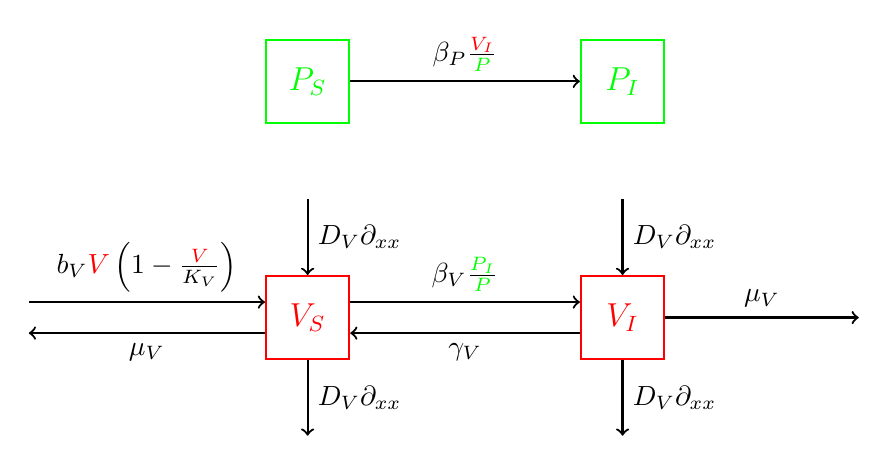
\begin{tikzpicture}[
    thick,
    scale = 1,
    %
    compartment/.style = {draw,
      font = \large,
      minimum size = {3em}},
    %
    plant/.style = {green},
    vector/.style = {red},
    ]

    \node at (0, 0)
    [compartment, vector, name = V_S] {$V_S$};
    \node at (4, 0)
    [compartment, vector, name = V_I] {$V_I$};

    \node at (0, 3)
    [compartment, plant, name = P_S] {$P_S$};
    \node at (4, 3)
    [compartment, plant, name = P_I] {$P_I$};

    \draw [->] (P_S) to node [above]
    {$\beta_P \frac{\textcolor{red}{V_I}}{\textcolor{green}{P}}$}
    (P_I);

    \draw [->] (V_S.20) to node [above]
    {$\beta_V \frac{\textcolor{green}{P_I}}{\textcolor{green}{P}}$}
    (V_I.160);

    \draw [->] (V_I.200) to node [below] {$\gamma_V$} (V_S.340);

    \draw [<-] (V_S.160) to node [above]
    {$b_V \textcolor{red}{V} \left(1 - \frac{\textcolor{red}{V}}{K_V}\right)$}
    +(180: 3);

    \draw [->] (V_S.200) to node [below] {$\mu_V$} +(180: 3);

    \draw [->] (V_I) to node [above] {$\mu_V$} +(0: 3);

    \draw [<-] (V_S) to node [right] {$D_V \partial_{xx}$} +(90: 1.5);

    \draw [->] (V_S) to node [right] {$D_V \partial_{xx}$} +(270: 1.5);

    \draw [<-] (V_I) to node [right] {$D_V \partial_{xx}$} +(90: 1.5);

    \draw [->] (V_I) to node [right] {$D_V \partial_{xx}$} +(270: 1.5);

  \end{tikzpicture}
  \caption{Model diagram.  $P_S$ and $P_I$ (green) are the densities
    of uninfected and plants.  $V_S$ and $V_I$ (red) are densities of
    uninfected and infected vectors.}
\end{figure}

The total plant density is constant in time,
$\frac{\partial P}{\partial t}(x, t) = \frac{\partial
  P_S}{\partial
  t}(x,
t) + \frac{\partial P_I}{\partial t}(x, t) = 0$,
so
$P(x, t) = P_S(x, t) + P_I(x, t) \implies P_S(x, t) = P(x, t) - P_I(x,
t)$.  Thus
\begin{equation}
  \label{pdesystemdimensional}
  \begin{split}
    \frac{\partial V_S}{\partial t}
    &= - \beta_V \frac{P_I}{P} V_S
    + \gamma_V V_I
    - \mu_V V_S
    + b_V V \left(1 - \frac{V}{K_V}\right)
    + D_V \frac{\partial^2 V_S}{\partial x^2},
    \\
    \frac{\partial V_I}{\partial t}
    &= \beta_V \frac{P_I}{P} V_S
    - \gamma_V V_I
    - \mu_V V_I
    + D_V \frac{\partial^2 V_I}{\partial x^2},
    \\
    \frac{\partial P_I}{\partial t}
    &= \beta_P V_I \left(1 - \frac{P_I}{P}\right).
  \end{split}
\end{equation}

We are initially thinking that the effects of the second insect
species will be
\begin{equation}
  \begin{split}
    \mu_V(r) &= \overline{\mu_V} (1 + \epsilon_{\mu_V} r),
    \\
    D_V(r) &= \overline{D_V} (1 + \epsilon_{D_V} r),
    \\
    \gamma_V(r) &= \overline{\gamma_V},
    \\
    b_V(r) &= \overline{b_V},
    \\
    K_V(r) &= \overline{K_V}.
  \end{split}
\end{equation}


\section{Nondimensionalization}

The disease-free spatially uniform steady state is
\begin{align}
  V_S = V^* &= K_V \left(1 - \frac{\mu_V}{b_V}\right),
  &
  V_I &= 0,
  &
  P_I &= 0.
\end{align}
We will use $V^*$ for the scale of $V_S$ and $V_I$, $\beta_V$ for the
time scale, and $\sqrt{\frac{\beta_V}{D_V}}$ for the spatial scale:
\begin{equation}
  \begin{aligned}
    \hat{V}_S &= \frac{V_S}{V^*},
    &
    \hat{V}_I &= \frac{V_I}{V^*},
    &
    \hat{P}_I &= \frac{P_I}{P},
    \\
    \hat{t} &= \beta_V t,
    &
    \hat{x} &= \sqrt{\frac{\beta_V}{D_V}} x,
    \\
    \hat{\beta}_P &= \frac{\beta_P}{\beta_V}\frac{V^*}{P},
    &
    \hat{\gamma}_V &= \frac{\gamma_V}{\beta_V},
    &
    \hat{b}_V &= \frac{b_V}{\beta_V},
    &
    \hat{\mu}_V &= \frac{\mu_V}{\beta_V},
  \end{aligned}
\end{equation}
Then
\begin{equation}
  \label{pdesystem}
  \begin{split}
    \frac{\partial \hat{V}_S}{\partial \hat{t}}
    &= - \hat{P}_I \hat{V}_S
    + \hat{\gamma}_V \hat{V}_I
    - \hat{\mu}_V \hat{V}_S
    + \hat{b}_V \hat{V} \left[1 - \left(1 - \frac{\hat{\mu}_V}{\hat{b}_V}\right) \hat{V}\right]
    + \frac{\partial^2 \hat{V}_S}{\partial \hat{x}^2},
    \\
    \frac{\partial \hat{V}_I}{\partial \hat{t}}
    &= \hat{P}_I \hat{V}_S
    - \hat{\gamma}_V \hat{V}_I
    - \hat{\mu}_V \hat{V}_I
    + \frac{\partial^2 \hat{V}_I}{\partial \hat{x}^2},
    \\
    \frac{\partial \hat{P}_I}{\partial \hat{t}}
    &= \hat{\beta}_P \hat{V}_I (1 - \hat{P}_I).
  \end{split}
\end{equation}

In what follows, we will drop the $\hat{}$, which hopefully won't
cause too much confusion.

\section{Wave-speed analysis}

We assume a solution that is a constant-shape wave traveling at speed
$c$.  The coordinate traveling with this wave is $z = x - c t$.  Let
\begin{equation}
  \begin{split}
    v_S(z) = v_S(x - c t) &= V_S(x, t),
    \\
    v_I(z) = v_I(x - c t) &= V_I(x, t),
    \\
    p_I(z) = p_I(x - c t) &= P_I(x, t).
  \end{split}
\end{equation}
Then \eqref{pdesystem} becomes
\begin{equation}
  \label{nonlinearode}
  \begin{split}
    - c \frac{\md v_S}{\md z}
    &= - p_I v_S 
    + \gamma_V v_I
    - \mu_V v_S
    + b_V v \left[1 - \left(1 - \frac{\mu_V}{b_V}\right) v\right]
    + \frac{\md^2 v_S}{\md z^2},
    \\
    - c \frac{\md v_I}{\md z}
    &= p_I v_S
    - \gamma_V v_I
    - \mu_V v_I
    + \frac{\md^2 v_I}{\md z^2},
    \\
    - c \frac{\md p_I}{\md z}
    &= \beta_P v_I (1 - p_I).
  \end{split}
\end{equation}
Converting this to a first-order system gives
\begin{equation}
  \label{nonlinear1storderode}
  \begin{split}
    \frac{\md v_S}{\md z} &= w_S,
    \\
    \frac{\md w_S}{\md z}
    &= \mu_V v_S
    - b_V v \left[1 - \left(1 - \frac{\mu_V}{b_V}\right) v\right]
    - c w_S - \gamma_V v_I + p_I v_S,
    \\
    \frac{\md v_I}{\md z} &= w_I,
    \\
    \frac{\md w_I}{\md z}
    &= (\gamma_V + \mu_V) v_I - c w_I - p_I v_S,
    \\
    \frac{\md p_I}{\md z}
    &= - \frac{\beta_P}{c} v_I (1 - p_I).
  \end{split}
\end{equation}

At the wave front, the susceptible vectors are at carrying capacity
and no infectious vectors or plants,
$v_S = 1$, $v_I = 0$, $p_I = 0$.
Linearizing \eqref{nonlinear1storderode} here gives
% \begin{equation}
%   \label{firstorderode}
%   \begin{split}
%     \frac{\md v_S}{\md z} &= w_S,
%     \\
%     \frac{\md w_S}{\md z}
%     &= 
%     (b_V - \mu_V) v_S - c w_S  - \gamma_V v_I + (b_V - 2 \mu_V) v_I + p_I,
%     \\
%     \frac{\md v_I}{\md z} &= w_I,
%     \\
%     \frac{\md w_I}{\md z}
%     &=  (\gamma_V + \mu_V) v_I - c w_I - p_I,
%     \\
%     \frac{\md p_I}{\md t}
%     &= - \frac{\beta_P}{c} v_I,
%   \end{split}
% \end{equation}
% or
\begin{equation}
  \frac{\md \vec{u}}{\md z}
  = \mat{A} \vec{u},
\end{equation}
with
\begin{align}
  \vec{u} &=
  \begin{pmatrix}
    v_S \\ w_S \\ v_I \\ w_I \\ p_I
  \end{pmatrix},
  &
  \mat{A} &=
  \begin{bmatrix}
    0 & 1 & 0 & 0 & 0
    \\
    b_V - \mu_V & - c & b_V - 2 \mu_V - \gamma_V & 0 & 1
    \\
    0 & 0 & 0 & 1 & 0 \\
    0 & 0 & \gamma_V + \mu_V & - c & - 1 \\
    0 & 0 & - \frac{\beta_P}{c} & 0 & 0
  \end{bmatrix}.
\end{align}

For a traveling wave, we need that all the eigenvalues of $\mat{A}$
are real.  Due to the $0$s in the bottom 3 entries of the left 2
columns, $\mat{A}$ is block diagonal and so its eigenvalues are
\begin{equation}
  \sigma(\mat{A}) = \sigma(\mat{A}_1) \cup \sigma(\mat{A}_2),
\end{equation}
with
\begin{align}
  \mat{A}_1 &=
  \begin{bmatrix}
    0 & 1 \\
    b_V - \mu_V & - c
  \end{bmatrix},
  &
  \mat{A}_2 &=
  \begin{bmatrix}
    0 & 1 & 0 \\
    \gamma_V + \mu_V & - c & - 1 \\
    - \frac{\beta_P}{c} & 0 & 0
  \end{bmatrix}.
\end{align}
The eigenvalues of $\mat{A}_1$ are
\begin{equation}
  \lambda = \frac{-c \pm \sqrt{c^2 + 4 (b_V - \mu_V)}}{2},
\end{equation}
which are always real provided that $b_V \geq \mu_V$, which is a
necessary condition for existence of the waves of interest.  The
characteristic equation for $\mat{A}_2$ is
\begin{subequations}
  \begin{equation}
    a_3 \lambda^3 + a_2 \lambda^2 +
    a_1 \lambda + a_0 = 0,
  \end{equation}
  with
  \begin{align}
    a_3 &= c, &
    a_2 &= c^2, &
    a_1 &= - c (\gamma_V + \mu_V), &
    a_0 &= - \beta_P.
  \end{align}
\end{subequations}
This has all real roots if the discriminant is non-negative:
\begin{equation}
  \begin{split}
    \Delta &=
    18 a_3 a_2 a_1 a_0
    - 4 a_2^3 a_0
    + a_2^2 a_1^2
    - 4 a_3 a_1^3
    - 27 a_3^2 a_0^2
    \\
    &= c^2 \Delta_1,
  \end{split}
\end{equation}
with
\begin{equation}
  \Delta_1
  =
  \left[(\gamma_V + \mu_V)^2 + 4 \beta_P\right] c^4
  + 2 (\gamma_V + \mu_V)
  \left[2 (\gamma_V + \mu_V)^2 + 9 \beta_P\right] c^2
  - 27 \beta_P^2.
\end{equation}
The discriminant is non-negative if $c = 0$ or $\Delta_1 = 0$.  For
$c = 0$, we have $v_I = 0$, which is the stationary disease-free
equilibrium, which is not the invasion wave of interest.  To find
where $\Delta_1 \geq 0$, we see that $\Delta_1 < 0$ at $c = 0$, so
$\Delta_1 \geq 0$ if
\begin{equation}
  c^2 \geq 
  \frac{2 \left[(\gamma_V + \mu_V)^2 + 3 \beta_P\right]^{3/2}
    - (\gamma_V + \mu_V) \left[2 (\gamma_V + \mu_V)^2 + 9 \beta_P\right]}
  {(\gamma_V + \mu_V)^2 + 4 \beta_P}
  > 0
\end{equation}
which is
\begin{equation}
  \label{speedcondition}
  |c| \geq
  \sqrt{\frac{2 \left[(\gamma_V + \mu_V)^2 + 3 \beta_P\right]^{3/2}
      - (\gamma_V + \mu_V) \left[2 (\gamma_V + \mu_V)^2 + 9 \beta_P\right]}
    {(\gamma_V + \mu_V)^2 + 4 \beta_P}}.
\end{equation}

The usual theory says that the emergent wave speed is the minimum one
that satisfies \eqref{speedcondition} (although I need to check that the
``cooperativity'' conditions of Weinberger et al are satisfied):
\begin{equation}
  c^* = \pm \sqrt{\frac{2 \left[(\gamma_V + \mu_V)^2 + 3 \beta_P\right]^{3/2}
      - (\gamma_V + \mu_V) \left[2 (\gamma_V + \mu_V)^2 + 9 \beta_P\right]}
    {(\gamma_V + \mu_V)^2 + 4 \beta_P}}.
\end{equation}


% \subsection{Invasion wave of vectors}

% At the wave front, there are no vectors and no infectious plants:
% $v_S = v_I = p_I = 0$.  Linearizing \eqref{nonlinear1storderode}
% here gives
% \begin{equation}
%   \label{firstorderode0}
%   \begin{split}
%     \frac{\md v_S}{\md z} &= w_S,
%     \\
%     \frac{\md w_S}{\md z}
%     &= (1 - b_V) v_S - c w_S - (\gamma_V + b_V) v_I
%     \\
%     \frac{\md v_I}{\md z} &= w_I,
%     \\
%     \frac{\md w_I}{\md z}
%     &= (1 + \gamma_V) v_I - c w_I,
%     \\
%     \frac{\md p_I}{\md t}
%     &= - \frac{\beta_P}{c} v_I,
%   \end{split}
% \end{equation}
% or
% \begin{equation}
%   \frac{\md}{\md z}
%   \begin{pmatrix}
%     v_S \\ w_S \\ v_I \\ w_I \\ p_I
%   \end{pmatrix}
%   = \mat{A}
%   \begin{pmatrix}
%     v_S \\ w_S \\ v_I \\ w_I \\ p_I
%   \end{pmatrix},
% \end{equation}
% with
% \begin{equation}
%   \mat{A} =
%   \begin{bmatrix}
%     0 & 1 & 0 & 0 & 0 \\
%     1 - b_V & - c & - b_V - \gamma_V & 0 & 0 \\
%     0 & 0 & 0 & 1 & 0 \\
%     0 & 0 & 1 + \gamma_V & - c & 0 \\
%     0 & 0 & - \frac{\beta_P}{c} & 0 & 0
%   \end{bmatrix}.
% \end{equation}
% To have a wave, we need all real eigenvalues of $\mat{A}$.  The
% eigenvalues of $\mat{A}$ are
% $\sigma(\mat{A}) = \{0\} \cup \sigma(\mat{A}_1) \cup
% \sigma(\mat{A}_2)$,
% where
% \begin{align}
%   \mat{A}_1 &=
%   \begin{bmatrix}
%     0 & 1 \\
%     1 - b_V & - c
%   \end{bmatrix},
%   &
%   \mat{A}_2 &=
%   \begin{bmatrix}
%     0 & 1 \\
%     1 + \gamma_V & - c
%   \end{bmatrix}.
% \end{align}
% These have eigenvalues
% \begin{equation}
%   \begin{split}
%     \sigma(\mat{A}_1) &= \left\{
%       \frac{-c \pm \sqrt{c^2 - 4 (b_v - 1)}}{2}
%     \right\},
%     \\
%     \sigma(\mat{A}_2) &= \left\{
%       \frac{-c \pm \sqrt{c^2 + 4 (1 + \gamma_V)}}{2}
%     \right\}.
%   \end{split}
% \end{equation}
% The eigenvalues of $\mat{A}_2$ are always real.  The eigenvalues of
% $\mat{A}_1$ are real if
% \begin{equation}
%   \label{wavespeed}
%   |c| \geq 2 \sqrt{b_v - 1}.
% \end{equation}
% The minimum wave speed is
% \begin{equation}
%   c^* = \pm 2 \sqrt{b_v - 1}.
% \end{equation}
% This is the usual invasion speed for a single species.



\section{Increasing $r$}

The wave speed in dimensional parameters is
\begin{equation}
  {c^*}^2 = D_V
    \frac{2 \left[(\gamma_V + \mu_V)^2 + 3 \beta V^*\right]^{3/2}
      - (\gamma_V + \mu_V) \left[2 (\gamma_V + \mu_V)^2 + 9 \beta V^*\right]}
    {(\gamma_V + \mu_V)^2 + 4 \beta V^*},
\end{equation}
where
\begin{align}
  V^* &= K_V \left(1 - \frac{\mu_V}{b_V}\right),
  &
  \beta &= \frac{\beta_P \beta_V}{P}.
\end{align}

We are initially thinking that the effects of the second insect
species will be on $\mu_V$ and $D_V$.  Differentiating
\begin{equation}
  \begin{split}
    \frac{\md {c^*}^2}{\md r}
    &=
    \frac{\md}{\md r} \left\{
      D_V
      \frac{2 \left[(\gamma_V + \mu_V)^2 + 3 \beta V^*\right]^{3/2}
        - (\gamma_V + \mu_V) \left[2 (\gamma_V + \mu_V)^2 + 9 \beta V^*\right]}
      {(\gamma_V + \mu_V)^2 + 4 \beta V^*}
    \right\},
    \\
    &=
    \left(
      \frac{\partial {c^*}^2}{\partial \mu_V}
      +
      \frac{\partial {c^*}^2}{\partial V^*} \frac{\md V^*}{\md \mu_V}
    \right)
    \frac{\md \mu_V}{\md r}
    +
    \frac{{c^*}^2}{D_V} \frac{\md D_V}{\md r},
    \\
    &=
    \left(
      \frac{\partial {c^*}^2}{\partial \mu_V}
      -
      \frac{K_V}{b_V}
      \frac{\partial {c^*}^2}{\partial V^*}
    \right)
    \mu_V \epsilon_{\mu_V}
    +
    {c^*}^2 \epsilon_{D_V},
  \end{split}
\end{equation}
with
\begin{equation}
  \begin{split}
    \frac{\partial {c^*}^2}{\partial \mu_V}
    &=
    D_V
    \frac{\partial}{\partial \mu_V} \left\{
      \frac{2 \left[(\gamma_V + \mu_V)^2 + 3 \beta V^*\right]^{3/2}
        - (\gamma_V + \mu_V) \left[2 (\gamma_V + \mu_V)^2 + 9 \beta V^*\right]}
      {(\gamma_V + \mu_V)^2 + 4 \beta V^*}
    \right\},
    % \\
    % &=
    % D_V
    % \frac{
    %   3 \left[
    %     2 (\gamma_V + \mu_V) \sqrt{(\gamma_V + \mu_V)^2 + 3 \beta V^*}
    %     - 2 (\gamma_V + \mu_V)^2 - 3 \beta V^*
    %   \right]
    %   \left[(\gamma_V + \mu_V)^2 + 4 \beta V^*\right]
    %   -
    %   2 (\gamma_V + \mu_V)
    %   \left\{
    %     2 \left[(\gamma_V + \mu_V)^2 + 3 \beta V^*\right]^{3/2}
    %     - (\gamma_V + \mu_V) \left[2 (\gamma_V + \mu_V)^2 + 9 \beta V^*\right]
    %   \right\}
    % }
    % {\left[(\gamma_V + \mu_V)^2 + 4 \beta V^*\right]^2},
    % \\
    % &=
    % {c^*}^2
    % \frac{
    %   3 \left[
    %     2 (\gamma_V + \mu_V) \sqrt{(\gamma_V + \mu_V)^2 + 3 \beta V^*}
    %     - 2 (\gamma_V + \mu_V)^2 - 3 \beta V^*
    %   \right]
    %   \left[(\gamma_V + \mu_V)^2 + 4 \beta V^*\right]
    %   -
    %   2 (\gamma_V + \mu_V)
    %   \left\{
    %     2 \left[(\gamma_V + \mu_V)^2 + 3 \beta V^*\right]^{3/2}
    %     - (\gamma_V + \mu_V) \left[2 (\gamma_V + \mu_V)^2 + 9 \beta V^*\right]
    %   \right\}
    % }
    % {\left[(\gamma_V + \mu_V)^2 + 4 \beta V^*\right]
    % \left\{2 \left[(\gamma_V + \mu_V)^2 + 3 \beta V^*\right]^{3/2}
    %   - (\gamma_V + \mu_V) \left[2 (\gamma_V + \mu_V)^2
    %     + 9 \beta V^*\right]\right\}},
    % \\
    % &=
    % {c^*}^2
    % \frac{
    %   2 (\gamma_V + \mu_V) \sqrt{(\gamma_V + \mu_V)^2 + 3 \beta V^*}
    %   \left[(\gamma_V + \mu_V)^2 + 6 \beta V^*\right]
    %   - 3 \left[2 (\gamma_V + \mu_V)^2 + 3 \beta V^*\right]
    %   \left[(\gamma_V + \mu_V)^2 + 4 \beta V^*\right]
    %   + 2 (\gamma_V + \mu_V)^2
    %   \left[2 (\gamma_V + \mu_V)^2 + 9 \beta V^*\right]
    % }
    % {\left[(\gamma_V + \mu_V)^2 + 4 \beta V^*\right]
    % \left\{2 \left[(\gamma_V + \mu_V)^2 + 3 \beta V^*\right]^{3/2}
    %   - (\gamma_V + \mu_V) \left[2 (\gamma_V + \mu_V)^2
    %     + 9 \beta V^*\right]\right\}},
    \\
    &=
    {c^*}^2
    \frac{
      2 \rho_V
      \left(\rho_V^2 + 6 \beta V^*\right)
      \sqrt{\rho_V^2 + 3 \beta V^*}
      - \left(
        2 \rho_V^4
        + 15 \beta V^* \rho_V^2
        + 36 \beta^2 {V^*}^2
      \right)
    }
    {\left(\rho_V^2 + 4 \beta V^*\right)
    \left[2 \left(\rho_V^2 + 3 \beta V^*\right)^{3/2}
      - \rho_V \left(2 \rho_V^2 + 9 \beta V^*\right)\right]},
  \end{split}
\end{equation}
\begin{equation}
  \begin{split}
    \frac{\partial {c^*}^2}{\partial V^*}
    &=
    D_V
    \frac{\partial}{\partial V^*} \left\{
      \frac{2 \left[(\gamma_V + \mu_V)^2 + 3 \beta V^*\right]^{3/2}
        - (\gamma_V + \mu_V) \left[2 (\gamma_V + \mu_V)^2 + 9 \beta V^*\right]}
      {(\gamma_V + \mu_V)^2 + 4 \beta V^*}
    \right\},
    % \\
    % &=
    % D_V
    % \frac{1}{\rho_V^2 + 4 \beta V^*}
    % \beta
    % \frac{
    %   9 \left(\sqrt{\rho_V^2 + 3 \beta V^*}
    %     - \rho_V\right)
    %   \left(\rho_V^2 + 4 \beta V^*\right)
    %   -
    %   4 \left[2 \left(\rho_V^2 + 3 \beta V^*\right)^{3/2}
    %     - \rho_V \left(2 \rho_V^2 + 9 \beta V^*\right)\right]
    % }
    % {\rho_V^2 + 4 \beta V^*},
    % \\
    % &=
    % {c^*}^2 \beta
    % \frac{
    %   9 \left(\sqrt{\rho_V^2 + 3 \beta V^*}
    %     - \rho_V\right)
    %   \left(\rho_V^2 + 4 \beta V^*\right)
    %   -
    %   4 \left[2 \left(\rho_V^2 + 3 \beta V^*\right)^{3/2}
    %     - \rho_V \left(2 \rho_V^2 + 9 \beta V^*\right)\right]
    % }
    % {\left(\rho_V^2 + 4 \beta V^*\right)
    %   \left[2 \left(\rho_V^2 + 3 \beta V^*\right)^{3/2}
    %     - \rho_V \left(2 \rho_V^2 + 9 \beta V^*\right)\right]},
    % \\
    % &=
    % {c^*}^2 \beta
    % \frac{
    %   9 \sqrt{\rho_V^2 + 3 \beta V^*} \left(\rho_V^2 + 4 \beta V^*\right)
    %   - 8 \sqrt{\rho_V^2 + 3 \beta V^*} \left(\rho_V^2 + 3 \beta V^*\right)
    %   - 9 \rho_V \left(\rho_V^2 + 4 \beta V^*\right)
    %   + 4 \rho_V \left(2 \rho_V^2 + 9 \beta V^*\right)
    % }
    % {\left(\rho_V^2 + 4 \beta V^*\right)
    %   \left[2 \left(\rho_V^2 + 3 \beta V^*\right)^{3/2}
    %     - \rho_V \left(2 \rho_V^2 + 9 \beta V^*\right)\right]},
    % \\
    % &=
    % {c^*}^2 \beta
    % \frac{
    %   \sqrt{\rho_V^2 + 3 \beta V^*} \left[
    %     9 \left(\rho_V^2 + 4 \beta V^*\right)
    %     - 8 \left(\rho_V^2 + 3 \beta V^*\right)
    %   \right]
    %   + \rho_V
    %   \left[4 \left(2 \rho_V^2 + 9 \beta V^*\right)
    %     - 9 \left(\rho_V^2 + 4 \beta V^*\right)
    %   \right]
    % }
    % {\left(\rho_V^2 + 4 \beta V^*\right)
    %   \left[2 \left(\rho_V^2 + 3 \beta V^*\right)^{3/2}
    %     - \rho_V \left(2 \rho_V^2 + 9 \beta V^*\right)\right]},
    % \\
    % &=
    % {c^*}^2 \beta
    % \frac{
    %   \sqrt{\rho_V^2 + 3 \beta V^*} \left(\rho_V^2 + 12 \beta V^*\right)
    %   - \rho_V^3
    % }
    % {\left(\rho_V^2 + 4 \beta V^*\right)
    %   \left[2 \left(\rho_V^2 + 3 \beta V^*\right)^{3/2}
    %     - \rho_V \left(2 \rho_V^2 + 9 \beta V^*\right)\right]},
    \\
    &=
    {c^*}^2 \beta
    \frac{\left(\rho_V^2 + 12 \beta V^*\right)
      \sqrt{\rho_V^2 + 3 \beta V^*} - \rho_V^3}
    {\left(\rho_V^2 + 4 \beta V^*\right)
      \left[2 \left(\rho_V^2 + 3 \beta V^*\right)^{3/2}
        - \rho_V \left(2 \rho_V^2 + 9 \beta V^*\right)\right]},
  \end{split}
\end{equation}
and
\begin{equation}
  \rho_V = \gamma_V + \mu_V.
\end{equation}


Alternately, in terms of semi-elasticities,
\begin{equation}
  \elasticity{y}{x}
  = \frac{1}{y} \frac{\partial y}{\partial x}
  = \frac{\partial \log y}{\partial x},
\end{equation}
we have
% \begin{equation}
%   \frac{1}{{c^*}^2}
%   \frac{\md {c^*}^2}{\md r}
%   =
%   \mu_V \left(
%     \frac{1}{{c^*}^2}
%     \frac{\partial {c^*}^2}{\partial \mu_V}
%     -
%     \frac{K_V}{b_V}
%     \frac{1}{{c^*}^2}
%     \frac{\partial {c^*}^2}{\partial V^*}
%   \right)
%   \frac{1}{\mu_V}
%   \frac{\md \mu_V}{\md r}
%   +
%   \frac{1}{D_V} \frac{\md D_V}{\md r},
% \end{equation}
\begin{equation}
  \begin{split}
    \elasticity{{c^*}^2}{r}
    &=
    \mu_V \left[
      \elasticity{{c^*}^2}{\mu_V}
      - \frac{K_V}{b_V} \elasticity{{c^*}^2}{V^*}
    \right]
    \elasticity{\mu_V}{r}
    +
    \elasticity{D_V}{r}
    \\
    &=
    \mu_V \left[
      \elasticity{{c^*}^2}{\mu_V}
      - \frac{K_V}{b_V} \elasticity{{c^*}^2}{V^*}
    \right]
    \epsilon_{\mu_V}
    +
    \epsilon_{D_V},
  \end{split}
\end{equation}
with
\begin{equation}
  % \frac{1}{{c^*}^2} \frac{\partial {c^*}^2}{\partial \mu_V}
  % =
  \elasticity{{c^*}^2}{\mu_V}
  =
  \frac{
    2 \rho_V \left(\rho_V^2 + 6 \beta V^*\right)
    \sqrt{\rho_V^2 + 3 \beta V^*}
    - \left(
      2 \rho_V^4
      + 15 \beta V^* \rho_V^2
      + 36 \beta^2 {V^*}^2
    \right)
  }
  {\left(\rho_V^2 + 4 \beta V^*\right)
    \left[2 \left(\rho_V^2 + 3 \beta V^*\right)^{3/2}
      - \rho_V \left(2 \rho_V^2 + 9 \beta V^*\right)\right]},
\end{equation}
and
\begin{equation}
  % \frac{1}{{c^*}^2} \frac{\partial {c^*}^2}{\partial V^*}
  % =
  \elasticity{{c^*}^2}{V^*}
  =
  \beta
  \frac{\left(\rho_V^2 + 12 \beta V^*\right)
    \sqrt{\rho_V^2 + 3 \beta V^*} - \rho_V^3}
  {\left(\rho_V^2 + 4 \beta V^*\right)
    \left[2 \left(\rho_V^2 + 3 \beta V^*\right)^{3/2}
      - \rho_V \left(2 \rho_V^2 + 9 \beta V^*\right)\right]}.
\end{equation}


\subsection{Negative elasticity}

When is $\elasticity{{c^*}^2}{r} < 0$?  This is
\begin{equation}
  \frac{\epsilon_{D_V}}{\epsilon_{\mu_V}}
  <
  \frac{\mu_V}{b_V}
  \frac{
    K_V 
    \beta
    \left[\left(\rho_V^2 + 12 \beta V^*\right)
      \sqrt{\rho_V^2 + 3 \beta V^*} - \rho_V^3\right]
    -
    2 b_V \rho_V \left(\rho_V^2 + 6 \beta V^*\right)
    \sqrt{\rho_V^2 + 3 \beta V^*}
    + b_V \left(
      2 \rho_V^4
      + 15 \beta V^* \rho_V^2
      + 36 \beta^2 {V^*}^2
    \right)}
  {\left(\rho_V^2 + 4 \beta V^*\right)
    \left[2 \left(\rho_V^2 + 3 \beta V^*\right)^{3/2}
      - \rho_V \left(2 \rho_V^2 + 9 \beta V^*\right)\right]}.
\end{equation}
\begin{equation}
  \frac{\epsilon_{D_V}}{\epsilon_{\mu_V}}
  <
  \frac{\mu_V}{b_V}
  \frac{
    \left[
      K_V
      \beta
      \left(\rho_V^2 + 12 \beta V^*\right)
      - 2 b_V \rho_V
      \left(\rho_V^2 + 6 \beta V^*\right)
    \right]
    \sqrt{\rho_V^2 + 3 \beta V^*}
    - K_V \beta \rho_V^3
    + b_V \left(
      2 \rho_V^4
      + 15 \beta V^* \rho_V^2
      + 36 \beta^2 {V^*}^2
    \right)}
  {\left(\rho_V^2 + 4 \beta V^*\right)
    \left[2 \left(\rho_V^2 + 3 \beta V^*\right)^{3/2}
      - \rho_V \left(2 \rho_V^2 + 9 \beta V^*\right)\right]}.
\end{equation}



% \section{1 species}

% \begin{equation}
%   \frac{\partial U}{\partial t}
%   = b U \left(1 - \frac{U}{K}\right)
%   - \mu U
%   + D \frac{\partial^2 U}{\partial x^2}
% \end{equation}
  
% Traveling wave: $z = x - c t$, $U(x, t) = u(z)$,
% \begin{equation}
%   - c \frac{\md u}{\md z}
%   = b u \left(1 - \frac{u}{K}\right)
%   - \mu u
%   + D \frac{\md^2 u}{\md z^2}
% \end{equation}

% Linearizing: $u = 0$
% \begin{equation}
%   - c \frac{\md u}{\md z}
%   =
%   (b - \mu) u
%   + D \frac{\md^2 u}{\md z^2}
% \end{equation}

% First order:
% \begin{equation}
%   \begin{split}
%     \frac{\md u}{\md z} &= w
%     \\
%     \frac{\md w}{\md z}
%     &=
%     - \frac{b - \mu}{D} u
%     - \frac{c}{D} w
%   \end{split}
% \end{equation}
% or
% \begin{equation}
%   \frac{\md \vec{y}}{\md z}
%   =
%   \begin{bmatrix}
%     0 & 1 \\
%     - \frac{b - \mu}{D} & - \frac{c}{D}
%   \end{bmatrix}
%   \vec{y}
% \end{equation}

% The characteristic equation is
% \begin{equation}
%   D \lambda^2 + c \lambda + (b - \mu) = 0
% \end{equation}
% so
% \begin{equation}
%   \lambda = \frac{- c \pm \sqrt{c^2 - 4 D (b - \mu)}}{2 D}
% \end{equation}
% thus
% \begin{equation}
%   {c^*}^2 = 4 D (b - \mu)
% \end{equation}

% Now
% \begin{equation}
%   \begin{split}
%     \frac{\md {c^*}^2}{\md r}
%     &=
%     \frac{\partial {c^*}^2}{\partial D} \frac{\md D}{\md r}
%     + \frac{\partial {c^*}^2}{\partial b} \frac{\md b}{\md r}
%     + \frac{\partial {c^*}^2}{\partial \mu} \frac{\md \mu}{\md r}
%     \\
%     &=
%     4 (b - \mu) \frac{\md D}{\md r}
%     + 4 D \frac{\md b}{\md r}
%     - 4 D \frac{\md \mu}{\md r}
%     \\
%     &=
%     {c^*}^2 \left[
%       \frac{1}{D} \frac{\md D}{\md r}
%       + \frac{b}{b - \mu} \frac{1}{b} \frac{\md b}{\md r}
%       - \frac{\mu}{b - \mu} \frac{1}{\mu} \frac{\md \mu}{\md r}
%     \right]
%   \end{split}
% \end{equation}
% or
% \begin{equation}
%   \begin{split}
%     \elasticity{{c^*}^2}{r}
%     % =
%     % \frac{1}{{c^*}^2} \frac{\md {c^*}^2}{\md r}
%     % &=
%     % D \frac{1}{{c^*}^2} \frac{\partial {c^*}^2}{\partial D}
%     % \frac{1}{D} \frac{\md D}{\md r}
%     % + b \frac{1}{{c^*}^2} \frac{\partial {c^*}^2}{\partial b}
%     % \frac{1}{b} \frac{\md b}{\md r}
%     % + \mu \frac{1}{{c^*}^2} \frac{\partial {c^*}^2}{\partial \mu}
%     % \frac{1}{\mu} \frac{\md \mu}{\md r}
%     % \\
%     &=
%     D \elasticity{{c^*}^2}{D} \elasticity{D}{r}
%     + b \elasticity{{c^*}^2}{b} \elasticity{b}{r}
%     + \mu \elasticity{{c^*}^2}{\mu} \elasticity{\mu}{r}
%     \\
%     &=
%     \elasticity{D}{r}
%     + \frac{b}{b - \mu} \elasticity{b}{r}
%     - \frac{\mu}{b - \mu} \elasticity{\mu}{r}
%     \\
%     &=
%     \elasticity{D}{r}
%     + \frac{b \elasticity{b}{r}
%       - \mu \elasticity{\mu}{r}}{b - \mu} 
%   \end{split}
% \end{equation}

% For example,
% \begin{align}
%   \elasticity{b}{r} &= 0,
% \end{align}
% then
% \begin{equation}
%   \elasticity{{c^*}^2}{r} 
%   =
%   \elasticity{D}{r} - \frac{\mu}{b - \mu} \elasticity{\mu}{r}
% \end{equation}

\section{Other ideas}

\begin{enumerate}
\item Explicitly model interacting species: $r = X(x, t)$ and then
  some reaction--diffusion equation for $X(x, t)$.
\item The diffusion rate should be density dependent:
  $D_V\big(r, V(x, t)\big)$ or even
  $D_V\big(r, V_S(x, t), V_I(x, t)\big)$.
\item Currently, we have forces of infection
  $\lambda_V = \beta_V \frac{P_I}{P}$ and
  $\lambda_P = \beta_P \frac{V_I}{P}$.  Instead incorporate uninfected
  and infected vector preference for infected and uninfected plants:
  $\lambda_V = \beta_V \frac{a_1 P_I}{P_S + a_1 P_I}$ and
  $\lambda_P = \beta_P \frac{a_2 V_I}{a_2 P_S + P_I}$.
\item \sout{The loss of infection in vectors.}  Done.
\item Exposed classes for vectors and plants.  Does this give gamma
  distributed probability of transmission vs.~time from one vector to
  one plant?  Do I need a pre-transmission stage instead?
\item Separate nymph and adult classes of vectors.
\item Separate stationary, feeding, transmitting vectors and moving
  vectors.
\item Separate crawling and flying vectors.
\end{enumerate}

\end{document}
